\section{Theorie}
\label{sec:Theorie}

Ein Stoff kann in drei verschiedenen Phasen, auch Aggregatzustände genannt, vorliegen.
Wie in der Zustandskurve (Abbildung:\ref{fig:zustand}) zu sehen, können in den abgegrenzten
Bereichen alle zugehörigen $p-$ und $T-$ Werte angenommen werden, die Linien
beschreiben die Übergänge der einzelnen Phasen. In der Nähe der Linien existieren zwei
Phasen nebeneinander. In diesem Versuch wird sich mit der Dampfdruckkurve beschaftigt, diese
liegt zwischen den Punkten $T.P.$ und $K.P.$.
\begin{figure}
 \centering
 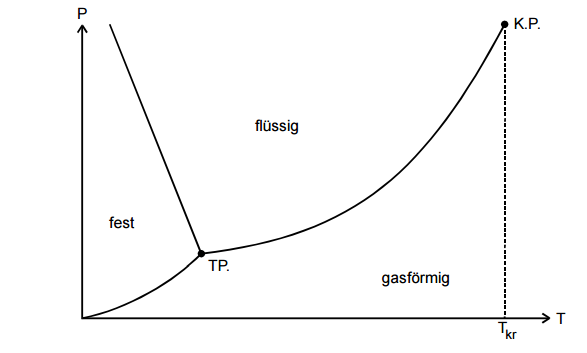
\includegraphics[width=0.7\textwidth]{zustand.png}
 \caption{Qualitatives Zustandsdiagramm von Wasser.}
 \label{fig:zusatnd}
 \end{figure}\\
 Die Form dieser Kurve ist durch die Verdampfungswärme $L$ bestimmt, diese ist notwendig um
 ein Mol einer Flüssigkeit in Dampf gleicher Temperatur umzuwandeln. Die größe $L$ ist
 temperaturabhängig, kann aber in bestimmten Bereichen als konstant angesehen werden.
 Beim Umwandlungsvorgang verlassen die Moleküle, die laut der Maxwellwellschen
 Geschwindigkeitsverteilung maximale kinetische Energie besitzen, die Flüssigkeitsoberfläche
 und gehen über in die gasförmige Phase. Um die Energie aufzubringen, die benötigt wird um
 die Bindungskräfte zu überwinden, muss entweder Energie von außen zugeführt weren oder
 der Flüssigkeit Wärme entzogen werden. Die entzogene Wärme wird bei der Kondensation des
 Gases wieder frei. Nach einiger Zeit stellt sich ein Gleichgewicht ein, es kehrt ebenso
 viel Flüssigkeit bei der Kondensation ins System zurück wie auch verdampft wird.
 In dem Gleichgewichtszustand herrscht der sogenannte Sättigungsdruck.
 Der Sättigungsdruck ist nicht abhängig vom Volumen des Gasraumes, daher lässt dieser sich durch
 die ideale Gasgleichung beschreiben:
 \begin{align}
 \rho V =RT
 \end{align}
 mit R als allgemeine Gaskonstante.
 \subsection{Herleitung der DGL für die Dampfdruckkurve}
Um die Dampfdruckkurve zu ermitteln, wird der reversible Kreisprozess der
Verdampfung und anschließender Kondensation zur Hilfe genommen.
In Abbildung \ref{fig:kreisprozess} ist der Kreisprozess qualitativ dargestellt.
\begin{figure}
 \centering
 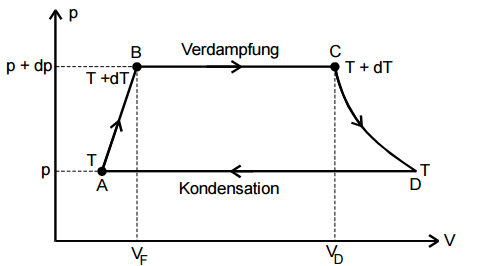
\includegraphics[width=0.7\textwidth]{kreisprozess.png}
 \caption{Kreisprozess im pV-Diagramm. }
 \label{fig:kreisprozess}
 \end{figure}\\
Zu Beginn wird ein Mol einer Flüssigkeit um die Temperatur $dT$ erwärmt, es steigt ebenfalls
der Druck um $dp$ und das Volumen auf $V_\mathrm{F}$. Dies entspricht dem Übergang $A\longrightarrow B$.
Beim Übergang $B\longrightarrow C$ geht die Wassermenge,nach Zufuhr der Verdampfungswärme, isobar
und isotherm in Gas über, dabei erweitert sich das Volumen auf $V_\mathrm{D}$.
Im Übergang $C \longrightarrow D$ kühlt sich der Dampf um $dT$ ab und der Druck
fallt ebenfalls zurück auf $p$. Im letzten Übergang $D\longrightarrow A$ wird die
Verdampfungswärme wieder freigesetzt, die Wassermenge kondensiert isobar und isotherm.
Die geleistete Arbeit wird mit der gesammt Wärmeenergie des Prozesses gleichgesetzt,
es ergibt sich folgende Gleichung:
\begin{align}
(C_\mathrm{F}-C_\mathrm{D})dT+dL=(V_\mathrm{D}-v\mathrm{F})dp.
\end{align}\\
Hier beschreiben $C_\mathrm{F}$ und $C_\mathrm{V}$ die Molwärmen im flüssigen und
gasförmigen Zustand und $V_\mathrm{F}$ und $V_\mathrm{D} die Volumina von Flüssigkeit und Dampf$.
Mit dem zweiten Hauptsatz der Thermodynamik:
\begin{align}
\sum_{i}\frac{Q_i}{T_i}=0
\end{align}
und weiteren Umformungen ergibt sich die Clausius-Clapeyronsche Gleichung:
\begin{align}
(V_\mathrm{D}-V_\mathrm{F})dp=\frac{L}{T}dT\label{eqn:clausius}.
\end{align}
